\documentclass[10pt,aspectratio=169]{beamer}

% Theme setup
\usetheme{metropolis}
\usecolortheme{default}

% Additional packages
\usepackage{booktabs}
\usepackage{tikz}
\usepackage{pgfplots}
\usepackage{xcolor}

% Define colors
\definecolor{placeholder}{RGB}{200,200,200}

% Keep the original title structure but update authors
\title{PVFinder for Real-Time Primary Vertexing at LHCb}
\subtitle{Hybrid DNN PV reconstruction for 30 MHz triggers at LHCb}
\author{Mohamed Elashri$^{1*}$, Simon Akar$^2$, Conor Henderson$^1$, Michael David Sokoloff$^1$ \\[0.3cm]
        {\small $^1$University of Cincinnati (US)} \\
        {\small $^2$LPCA - Université Clermont Auvergne (FR)} \\
        {\small $^*$Corresponding author}}
\date{\textbf{7th Inter-Experimental LHC Machine Learning Workshop} \\[0.2cm] \today}

\begin{document}

% Title slide
\begin{frame}
  \titlepage
  
  % Add some space and position content at bottom
  \vspace{-2cm}
  
  \begin{columns}[b]
    \begin{column}{0.55\textwidth}
      \raggedright
      {\footnotesize \textit{This work is supported by IRIS-HEP}}
    \end{column}
    
    \begin{column}{0.45\textwidth}
      \raggedleft
      
\includegraphics[height=0.9cm]{figures/iris-hep-logo.png} \;
      
\includegraphics[height=0.9cm]{figures/uc-logo.png} \;
      
\includegraphics[height=0.9cm]{figures/lhcb-logo.jpg} \;
      
\includegraphics[height=0.9cm]{figures/cern-logo.png}
    \end{column}
  \end{columns}
  
  \vspace{0.3cm}
\end{frame}

% Slide 2: Why Fast PVs in LHCb Run 3?
\begin{frame}{Why Fast PVs in LHCb Run 3?}
  \begin{itemize}
    \item LHCb detector upgraded for Run 3 with \textbf{5-fold increase} in luminosity
    \item Pure software trigger requires fast, accurate PV reconstruction
    \item Flavour physics selections critically depend on prompt z$_{\text{PV}}$
    \item Strict latency budget: \textbf{$\approx$ 200 $\mu$s} total processing time
  \end{itemize}

  \begin{center}
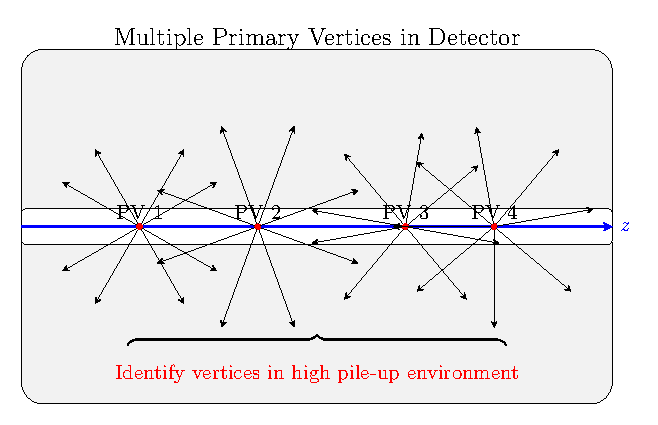
\includegraphics[width=0.35\textwidth]{figures/pvs.pdf}
\end{center}

  \pause
  \vspace{-0.3cm}
  \textbf{Challenge:} Reconstruct all primary vertices at 30 MHz with high efficiency
\end{frame}

% Slide 3: LHCb Trigger Chain
\begin{frame}{LHCb Trigger Chain}
  \begin{columns}[T]
    \begin{column}{0.6\textwidth}
      \textbf{Run 3: }
      \begin{itemize}
        \item \textbf{Allen (GPU)} first-level trigger (30 MHz)
        \item Processing $\sim$40 Tbit/s raw data
        \item Triggerless readout to event building servers
        \item Full selection in software - no hardware trigger
      \end{itemize}
    \end{column}

    \begin{column}{0.4\textwidth}
      \begin{center}
        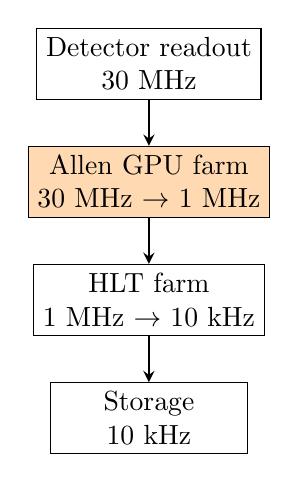
\begin{tikzpicture}[
          box/.style={draw, minimum width=2.5cm, minimum height=0.8cm, align=center}
        ]
          \node[box] (raw) at (0,0) {Detector readout\\30 MHz};
          \node[box, fill=orange!30] (allen) at (0,-1.5) {Allen GPU farm\\30 MHz $\rightarrow$ 1 MHz};
          \node[box] (hlt) at (0,-3) {HLT farm\\1 MHz $\rightarrow$ 10 kHz};
          \node[box] (storage) at (0,-4.5) {Storage\\10 kHz};

          \draw[-stealth, thick] (raw) -- (allen);
          \draw[-stealth, thick] (allen) -- (hlt);
          \draw[-stealth, thick] (hlt) -- (storage);
        \end{tikzpicture}
      \end{center}
    \end{column}
  \end{columns}

  GPU farm: \textbf{$\sim$500 GPUs} hosted in event building servers\\
  First complete high-throughput GPU trigger in a HEP experiment
\end{frame}

% Slide 4: Inside Allen
\begin{frame}{Inside Allen}
  \begin{columns}[T]
    \begin{column}{0.58\textwidth}
      \small
      \textbf{Key Design Principles:}
      \begin{itemize}
        \item Structure of arrays data model
        \item CUDA streams for event slices
        \item Zero dynamic allocation; pre-allocated pools
        \item One event $\approx$ one block
        \item Intra-event parallelism mapped to threads
      \end{itemize}
      \vspace{0.3cm}
      \textbf{Allen Pipeline:}
      \begin{itemize}
        \item Track reconstruction (Velo, UT, SciFi)
        \item Vertex finding, muon ID, parameterized Kalman filter
        \item 1 MHz output with tracks \& vertices
      \end{itemize}
      \vspace{0.3cm}
      \textbf{Integration Challenge:} Adapt external libraries to Allen's thread/memory model
    \end{column}
    \begin{column}{0.42\textwidth}
      \begin{center}
        \href{https://arxiv.org/abs/1912.09161}{\textcolor{blue}{Allen GPU trigger paper (arXiv:1912.09161)}}
        \\
        \vspace{0.2cm}
        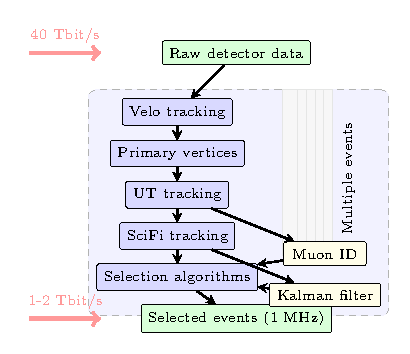
\includegraphics[width=0.95\textwidth]{figures/allen-workflow-compact.pdf}
      \end{center}
    \end{column}
  \end{columns}
\end{frame}


% Slide 5: PVFinder Concept
\begin{frame}{PVFinder Concept}
  \begin{columns}[T]
    \begin{column}{0.6\textwidth}
      \textbf{Evolution from traditional PV-finding:}
      \small
      \begin{itemize}
        \item Conventional: Heuristic track clustering
        \item PVFinder: End-to-end deep learning solution
        \item Hybrid approach:
          \begin{itemize}
            \item FC layers + CNN architecture
            \item Loss combines classification + regression
          \end{itemize}
        \item Adaptable across LHCb and ATLAS
      \end{itemize}
    \end{column}
    \begin{column}{0.4\textwidth}
      \begin{center}
        \href{https://arxiv.org/abs/2309.12417}{\textcolor{blue}{PVFinder paper (arXiv:2309.12417)}}
        \\
        \vspace{0.2cm}
        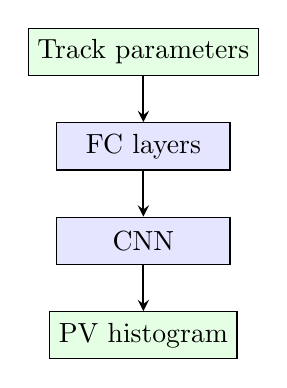
\begin{tikzpicture}[
          box/.style={draw, minimum width=2.2cm, minimum height=0.6cm, align=center},
        ]
          \node[box, fill=green!10] (tracks) at (0,0) {Track parameters};
          \node[box, fill=blue!10] (fcnn) at (0,-1.2) {FC layers};
          \node[box, fill=blue!10] (unet) at (0,-2.4) {CNN};
          \node[box, fill=green!10] (hist) at (0,-3.6) {PV histogram};
          \draw[-stealth, thick] (tracks) -- (fcnn);
          \draw[-stealth, thick] (fcnn) -- (unet);
          \draw[-stealth, thick] (unet) -- (hist);
        \end{tikzpicture}
      \end{center}
    \end{column}
  \end{columns}
  \vspace{-0.5cm}
  \small
  \textbf{Two-stage process:}
  \begin{enumerate}
    \item Track parameters → FC → latent "KDE-like" features
    \item → CNN → predicted target histogram → PV positions
  \end{enumerate}
\end{frame}

% Slide 6: Network Architecture
\begin{frame}{Network Architecture}
  \begin{center}
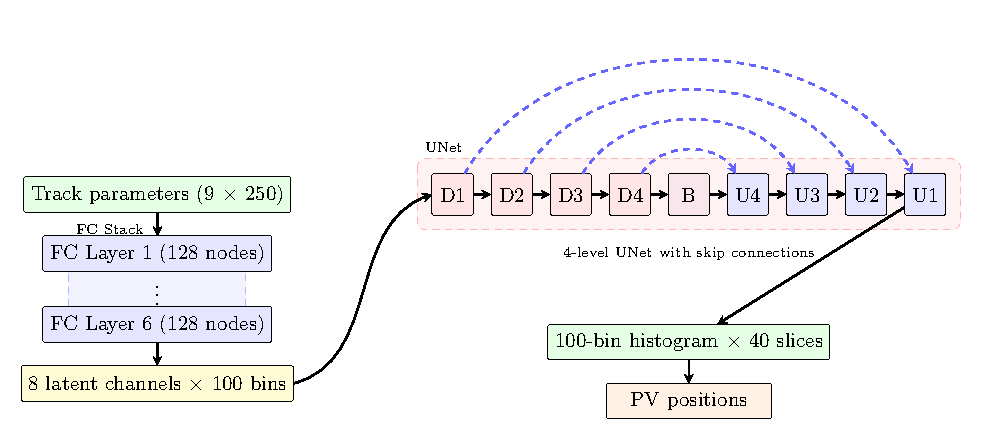
\includegraphics[width=0.75\textwidth]{figures/pvfinder-diagram-compact.pdf}  
  \end{center}

  \textbf{PVFinder algorithm steps:} 
  \begin{enumerate}
    \item \textbf{Spatial slicing:} Split detector z-region (4000 bins) into 40 intervals of 100 bins each
    \item \textbf{FC Network:} Process track parameters within each slice to create histogram-like features
    \item \textbf{CNN Network:} Process 1D histogram features with spatial context to predict PVs
  \end{enumerate}
\end{frame}

% Slide 7: LHCb Performance
\begin{frame}{LHCb Performance}
  \begin{columns}[T]
    \begin{column}{0.55\textwidth}
      \textbf{Key metrics:}
      \begin{itemize}
        \item \textbf{Efficiency:} $>$96\% (exceeds heuristic)
        \item \textbf{False positive rate:} 0.03 per event
        \item \textbf{Z-resolution:} $\sim$12 $\mu$m (competitive)
        \item \textbf{FP16 quantization:} minimal impact
        \item \textbf{CNN channels:} 16-64 explored
      \end{itemize}
    \end{column}

    \begin{column}{0.45\textwidth}
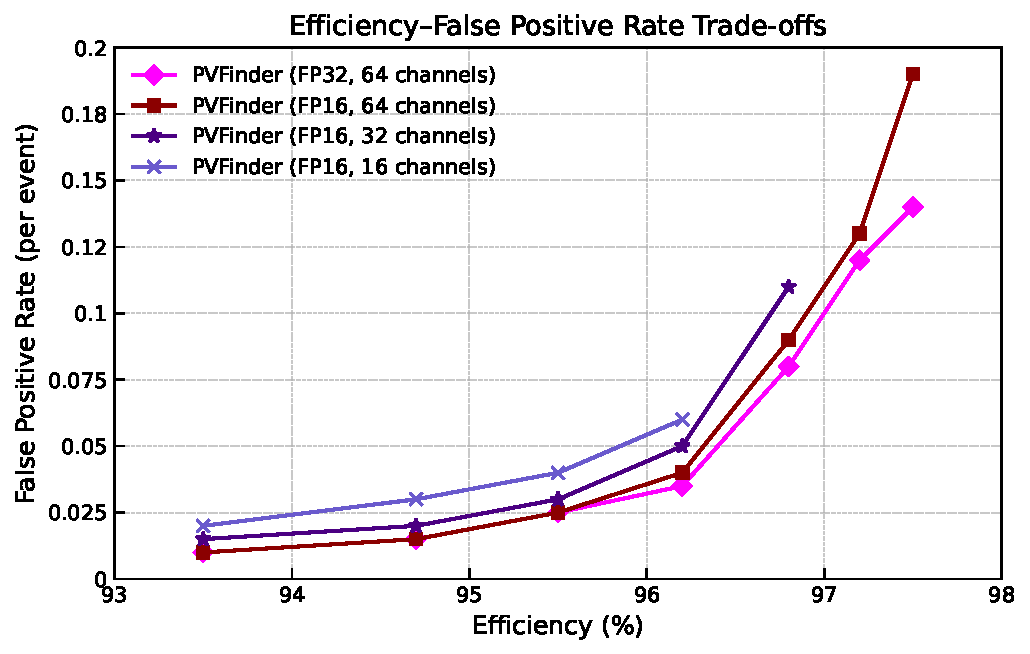
\includegraphics[width=1.0\textwidth]{figures/pvfinder_performance.pdf}
    \end{column}
  \end{columns}

  \pause
  \vspace{-0.1cm}
  \textbf{Achievement:} End-to-end tracks-to-hist model outperforms KDE-to-hist models
\end{frame}

% Slide 8: Embedding PVFinder in Allen: Requirements
\begin{frame}{Embedding PVFinder in Allen: Requirements}
  \begin{columns}[T]
    \begin{column}{0.58\textwidth}
      \textbf{Integration constraints:}
      \begin{itemize}
        \item 30 MHz input (33 $\mu$s/event)
        \item Latency budget: 150 $\mu$s kernel time
        \item Deterministic memory footprint
        \item Minimal external dependencies
        \item SoA data format compatibility
      \end{itemize}
      
      \textbf{Allen processing model:}
      \begin{itemize}
        \item Raw data copied to GPU once
        \item Full algorithm sequence on GPU
        \item Only selection results returned to CPU
      \end{itemize}
    \end{column}

    \begin{column}{0.42\textwidth}
      \begin{center}
        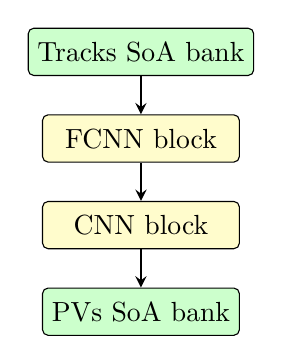
\begin{tikzpicture}[
          box/.style={draw, minimum width=2.5cm, minimum height=0.6cm, align=center, rounded corners=2pt},
        ]
          \node[box, fill=green!20] (tracks) at (0,0) {Tracks SoA bank};
          \node[box, fill=yellow!20] (fcnn) at (0,-1.1) {FCNN block};
          \node[box, fill=yellow!20] (cnn) at (0,-2.2) {CNN block};
          \node[box, fill=green!20] (pvs) at (0,-3.3) {PVs SoA bank};

          \draw[-stealth, thick] (tracks) -- (fcnn);
          \draw[-stealth, thick] (fcnn) -- (cnn);
          \draw[-stealth, thick] (cnn) -- (pvs);
        \end{tikzpicture}
      \end{center}
    \end{column}
  \end{columns}

  \vspace{-0.1cm}
  \textbf{Two-part implementation challenge:}
  \begin{enumerate}
    \item Custom FCNN implementation \textcolor{green}{\textbf{Completed}}
    \item CNN block with cuDNN integration \textcolor{orange}{\textbf{In progress}}
  \end{enumerate}
\end{frame}

% Slide 9: FCNN Inference Engine
\begin{frame}{FCNN Inference Engine (implemented)}
  \begin{columns}[T]
    \begin{column}{0.58\textwidth}
      \textbf{Implementation details:}
      \begin{itemize}
        \item Hand-written CUDA matrix-vector ops
        \item Zero external dependencies
        \item Native support for Allen SoA format
        \item Integration with Allen memory pools
      \end{itemize}

    \textbf{Performance:}
    \begin{itemize}
      \item \textbf{Impact:} Only 2.26 kHz reduction in throughput
      \item \textbf{Latency added:} ~0.5 $\mu$s/event on NVIDIA RTX 2080
      \item \textbf{Throughput maintained:} 96.8\% of baseline
    \end{itemize}
    \end{column}
    
    \begin{column}{0.45\textwidth}
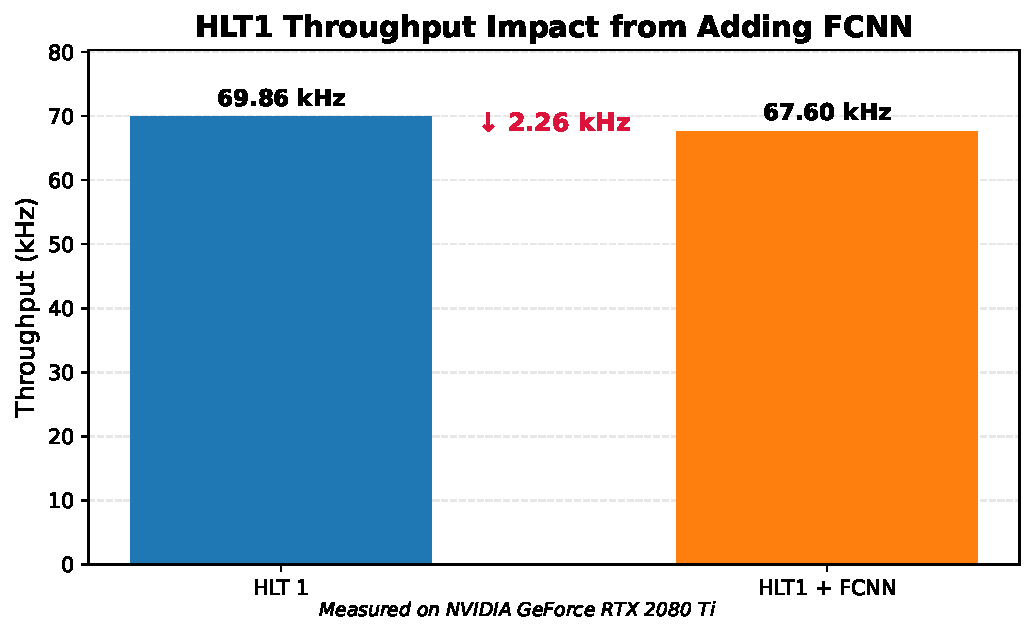
\includegraphics[width=1.1\textwidth]{figures/pvfinder_fcnn_impact.pdf}
    \end{column}
  \end{columns}

\end{frame}

% Slide 10: CNN Block Integration Challenges
\begin{frame}{CNN Block Integration Challenges}
  \begin{columns}[T]
    \begin{column}{0.58\textwidth}
      \textbf{Key integration issues:}
      \begin{itemize}
        \item \textbf{Format mismatch:} 
          \begin{itemize}
            \item cuDNN: NCHW tensor format
            \item Allen: SoA flat arrays
          \end{itemize}
        \item \textbf{Resource management:}
          \begin{itemize}
            \item Workspace memory ownership
            \item CUDA stream coordination
          \end{itemize}
        \item \textbf{Execution model:}
          \begin{itemize}
            \item Allen: async event-parallel
            \item cuDNN: blocking API calls
          \end{itemize}
      \end{itemize}
    \end{column}

    \begin{column}{0.42\textwidth}
      \begin{center}
        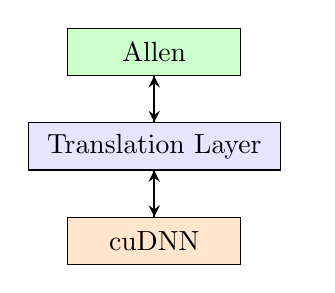
\begin{tikzpicture}[
          box/.style={draw, minimum width=2.2cm, minimum height=0.6cm, align=center},
          interface/.style={draw, fill=blue!10, minimum width=3.2cm, minimum height=0.6cm, align=center}
        ]
          \node[box, fill=green!20] (allen) at (0,0) {Allen};
          \node[interface] (trans) at (0,-1.2) {Translation Layer};
          \node[box, fill=orange!20] (cudnn) at (0,-2.4) {cuDNN};

          \draw[-stealth, thick] (allen) -- (trans);
          \draw[-stealth, thick] (trans) -- (cudnn);
          \draw[-stealth, thick] (cudnn) -- (trans);
          \draw[-stealth, thick] (trans) -- (allen);

          \node[anchor=west] at (1.7,-1.2) {
            \begin{minipage}{2.5cm}
            \end{minipage}
          };
        \end{tikzpicture}
      \end{center}
    \end{column}
  \end{columns}

  \textbf{Solution:} Translation layer with batch-amortized memory operations
\end{frame}

% Slide 11: NEW - Translation Layer Concept
\begin{frame}{Translation Layer: Bridging Allen and cuDNN}
  \begin{columns}[T]
    \begin{column}{0.4\textwidth}
      \textbf{The integration challenge:}
      \begin{itemize}
        \item Allen and cuDNN have fundamentally different:
          \begin{itemize}
            \item Memory models
            \item Data layouts
            \item Execution patterns
          \end{itemize}
      \end{itemize}
      
      \vspace{0.1cm}
      \textbf{Our solution:}
      \begin{itemize}
        \item Create an abstraction layer that acts as a bridge
        \item Handle all conversions and synchronization internally
        \item Present Allen-compatible interfaces to both sides
      \end{itemize}
    \end{column}

    \begin{column}{0.6\textwidth}
      \begin{center}
        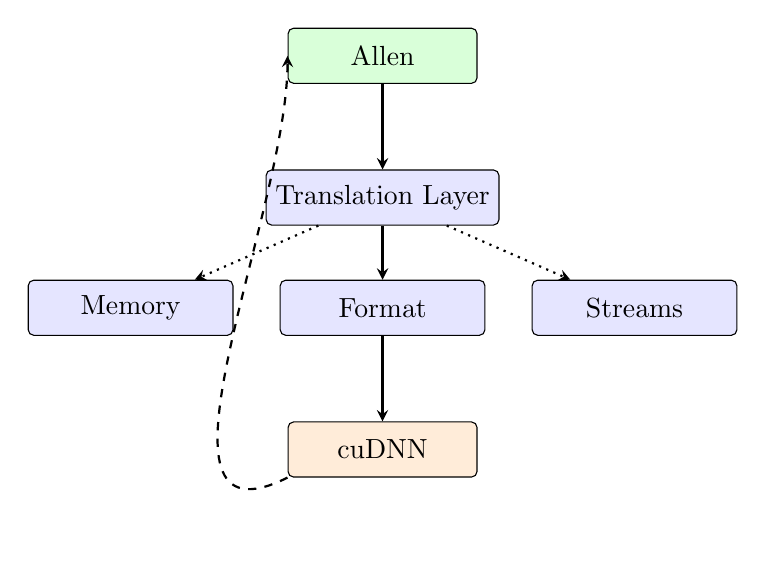
\begin{tikzpicture}[
          box/.style={draw, minimum width=2.4cm, minimum height=0.7cm, align=center, rounded corners=2pt},
          interface/.style={draw, fill=blue!10, minimum width=2.6cm, minimum height=0.7cm, align=center, rounded corners=2pt},
          arrow/.style={->, thick, >=stealth}
        ]
          % Allen Side
          \node[box, fill=green!15] (allen) at (0,0) {Allen};
          
          % Translation Layer
          \node[interface] (trans) at (0,-1.8) {Translation Layer};

          % Lower cuDNN
          \node[box, fill=orange!15] (cudnn) at (0,-5) {cuDNN};

          % Interfaces: memory, format, stream
          \node[interface] (memory) at (-3.2,-3.2) {Memory};
          \node[interface] (format) at (0,-3.2) {Format};
          \node[interface] (stream) at (3.2,-3.2) {Streams};

          % Main arrows
          \draw[arrow] (allen) -- (trans);
          \draw[arrow] (trans) -- (format);
          \draw[arrow] (format) -- (cudnn);

          % Diagonal dotted arrows to avoid overlap
          \draw[arrow, dotted] (trans) -- (memory);
          \draw[arrow, dotted] (trans) -- (stream);

          % Feedback path, now curved to avoid clutter
          \draw[arrow, dashed] (cudnn.south west) .. controls +(-2,-1) and +(0,-2) .. (allen.west);

        \end{tikzpicture}
      \end{center}
    \end{column}
  \end{columns}

\end{frame}

% Slide 12: NEW - Translation Layer Implementation Details
\begin{frame}{Translation Layer: Implementation Details}
  \begin{columns}[T]
    \begin{column}{0.48\textwidth}
      \textbf{Three-phase implementation:}
      \begin{enumerate}
        \item \textbf{Prepare Phase:}
           \begin{itemize}
             \item SoA track data → NCHW tensors
             \item Pre-allocated workspace setup
             \item Batch dimension mapping
           \end{itemize}
        \item \textbf{Execute Phase:}
           \begin{itemize}
             \item cuDNN neural network inference
             \item Event-parallel processing
             \item Non-blocking stream execution
           \end{itemize}
        \item \textbf{Extract Phase:}
           \begin{itemize}
             \item NCHW results → SoA format
             \item Memory cleanup and recycling
             \item Data transfer optimization
           \end{itemize}
      \end{enumerate}
    \end{column}
    
    \begin{column}{0.5\textwidth}
      \begin{center}
        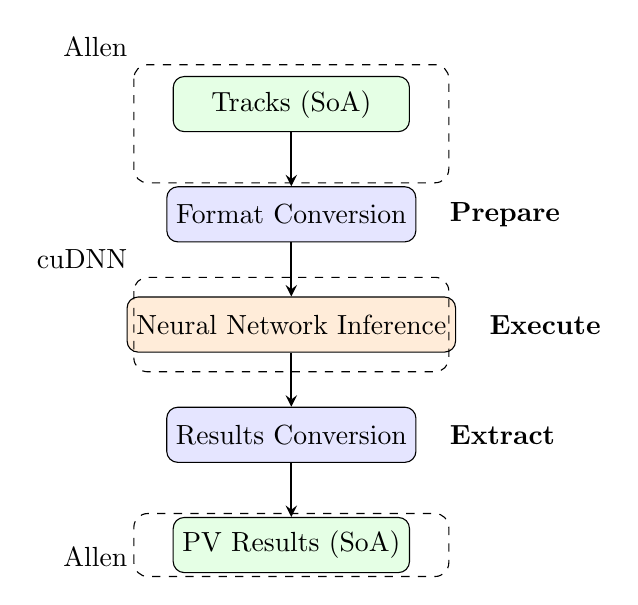
\begin{tikzpicture}[
          box/.style={draw, minimum width=3cm, minimum height=0.7cm, align=center, rounded corners},
          arrow/.style={->, thick, >=stealth},
          phase/.style={draw=none, right=0.3cm}
        ]
          % Allen Side
          \node[box, fill=green!10] (tracks) at (0,0) {Tracks (SoA)};
          
          % Phases with boxes
          \node[box, fill=blue!10] (prepare) at (0,-1.4) {Format Conversion};
          \node[phase] at (prepare.east) {\textbf{Prepare}};
          
          \node[box, fill=orange!15] (execute) at (0,-2.8) {Neural Network Inference};
          \node[phase] at (execute.east) {\textbf{Execute}};
          
          \node[box, fill=blue!10] (extract) at (0,-4.2) {Results Conversion};
          \node[phase] at (extract.east) {\textbf{Extract}};
          
          % Output
          \node[box, fill=green!10] (pvs) at (0,-5.6) {PV Results (SoA)};
          
          % Connections
          \draw[arrow] (tracks) -- (prepare);
          \draw[arrow] (prepare) -- (execute);
          \draw[arrow] (execute) -- (extract);
          \draw[arrow] (extract) -- (pvs);
          
          % Allen/cuDNN domains
          \draw[dashed, rounded corners=5pt] (-2,0.5) rectangle (2,-1.0) node[pos=0.01, above left] {Allen};
          \draw[dashed, rounded corners=5pt] (-2,-2.2) rectangle (2,-3.4) node[pos=0.01, above left] {cuDNN};
          \draw[dashed, rounded corners=5pt] (-2,-6.0) rectangle (2,-5.2) node[pos=0.01, above left] {Allen};
        \end{tikzpicture}
      \end{center}
    \end{column}
  \end{columns}
  
  \vspace{0.2cm}
  \textbf{Key advantages:}
  \begin{itemize}
    \item Isolates cuDNN dependencies from Allen codebase
    \item Maintains Allen's deterministic memory model
    \item Enables easy adaptation to other neural network libraries
  \end{itemize}
\end{frame}

% Summary slide
\begin{frame}{Summary}
  \textbf{Key Achievements:}
  \begin{itemize}
    \item \textbf{Algorithm Development:} End-to-end tracks-to-hist PVFinder with $>96\%$ efficiency
    \item \textbf{Performance:} False positive rate of 0.03 per event, competitive z-resolution
    \item \textbf{FCNN Implementation:} Custom CUDA engine integrated in Allen with minimal latency impact
    \item \textbf{Translation Layer:} Novel bridge architecture for Allen-cuDNN integration
  \end{itemize}

  \vspace{0.1cm}
  \textbf{Current Status:}
  \begin{itemize}
    \item FCNN inference engine: \textcolor{green}{\textbf{Completed}}
    \item Translation layer design: \textcolor{green}{\textbf{Completed}}  
    \item Full CNN integration: \textcolor{orange}{\textbf{Target Q3 2025}}
  \end{itemize}

  \vspace{0.1cm}
  \textbf{Impact:}
  \begin{itemize}
    \item First hybrid DNN approach for real-time PV reconstruction at 30 MHz
    \item Scalable framework for ML integration in high-throughput triggers
  \end{itemize}
\end{frame}

% Backup Slides transition
\begin{frame}[plain]
  \begin{center}
    \vspace{2cm}
    {\Huge\bfseries Thank you, Questions?}
    \vspace{2cm}
  \end{center}
\end{frame}



% Backup Slides transition
\begin{frame}[plain]
  \begin{center}
    \vspace{2cm}
    {\Huge\bfseries Backup Slides}
    \vspace{2cm}
  \end{center}
\end{frame}

% Moving Roadmap to Full Deployment to backup
\begin{frame}{Roadmap to Full Deployment}
  \begin{enumerate}
    \item \textbf{Finalize translation layer API} (Q2 2025)
      \begin{itemize}
        \item Complete abstraction shim between Allen and cuDNN
        \item Validate memory management approach
      \end{itemize}
    \item \textbf{Fuse histogram maker + CNN} (Q2-Q3 2025)
      \begin{itemize}
        \item Remove intermediate data copies
        \item End-to-end slice processing
      \end{itemize}
    \item \textbf{Harmonize memory pools} (Q3 2025)
      \begin{itemize}
        \item Integrate with Allen's allocation strategy
        \item Optimize for GPU cache usage
      \end{itemize}
    \item \textbf{End-to-end benchmark} (Q4 2025)
      \begin{itemize}
        \item Target: $<$ 120 $\mu$s total latency
        \item Measure throughput at scale
      \end{itemize}
    \item \textbf{Validation on 2025 data} (Q4 2025-Q1 2026)
  \end{enumerate}
\end{frame}

% Backup Slide 1: Translation Layer API Sketch
\begin{frame}{Backup: Translation Layer API Sketch}
  \begin{columns}[T]
    \begin{column}{0.55\textwidth}
      \small
\begin{verbatim}
// Translation layer header (simplified)
namespace pvfinder {
namespace allen_cudnn {

class TranslationLayer {
public:
  TranslationLayer(
    AllenMemoryPool& pool,
    const AllenConfig\& config);
    
  // Convert Allen SoA to cuDNN format
  void prepareInputTensor(
    const AllenBank\& input_bank);
    
  // Run CNN forward pass
  void forward(cudaStream_t stream);
    
  // Copy results back to Allen format
  void extractResults(
    AllenBank\& output_bank);

private:
  CudnnWorkspaceHandler m_workspace;
  TensorConverter m_converter;
  UNetConfig m_config;
};

} // namespace allen_cudnn
} // namespace pvfinder
\end{verbatim}
    \end{column}

    \begin{column}{0.45\textwidth}
      \textbf{Key design principles:}

      \begin{itemize}
        \item Clean separation of concerns
        \item Explicit memory ownership
        \item Non-blocking operations
        \item Minimal data copies
        \item Thread-safe execution
      \end{itemize}

      \textbf{Memory contract:}
      \begin{itemize}
        \item Pre-allocated workspace
        \item No dynamic allocations
        \item Fixed tensor shapes
        \item Reuse conversion buffers
      \end{itemize}
    \end{column}
  \end{columns}
\end{frame}

% Backup Slide 2: Detailed Latency Budget
\begin{frame}{Backup: Detailed Latency Budget}
  \begin{columns}[T]
    \begin{column}{0.5\textwidth}
      \textbf{Target latency breakdown:}
      \begin{center}
        \begin{tabular}{lr}
          \toprule
          \textbf{Component} \& \textbf{Budget ($\mu$s)} \\
          \midrule
          Input preparation \& 10 \\
          FCNN inference \& 7 \\
          Format conversion \& 15 \\
          CNN forward pass \& 70 \\
          Output conversion \& 10 \\
          Peak finding \& 8 \\
          \midrule
          \textbf{Total} \& \textbf{120} \\
          \bottomrule
        \end{tabular}
      \end{center}
    \end{column}

    \begin{column}{0.5\textwidth}
      \textbf{Performance targets:}
      \begin{itemize}
        \item 97\%+ efficiency
        \item $<$ 5\% false positive rate
        \item $<$ 150 $\mu$s average latency
        \item $<$ 200 $\mu$s worst-case latency
      \end{itemize}

      \vspace{0.5cm}
      \textbf{Allen context:}
      \begin{itemize}
        \item 30 MHz input rate
        \item 33 $\mu$s wall-time per event
        \item 150 $\mu$s kernel time budget
        \item Must maintain deterministic latency
      \end{itemize}
    \end{column}
  \end{columns}
\end{frame}


\end{document}